% SPDX-License-Identifier: CC-BY-4.0
% Copyright (c) 2026 Jonathan Yantis. Author-review research draft.
\documentclass[11pt,letterpaper]{article}
\usepackage[margin=.77in]{geometry}
\usepackage[T1]{fontenc}
\usepackage{lmodern,microtype,amsmath,amssymb,booktabs,array,ragged2e,xcolor,tikz,pgfplots,fancyhdr,xurl}
\usetikzlibrary{arrows.meta,positioning,calc}
\pgfplotsset{compat=1.18}
\definecolor{ink}{HTML}{24465B}\definecolor{pale}{HTML}{EDF2F3}\definecolor{amber}{HTML}{A85F2B}\definecolor{green}{HTML}{26705B}
\usepackage[colorlinks=true,allcolors=ink]{hyperref}
\setlength{\parindent}{0pt}\setlength{\parskip}{4pt}\setlength{\headheight}{14pt}\setlength{\emergencystretch}{2em}
\newcolumntype{L}[1]{>{\RaggedRight\arraybackslash}p{#1}}
\newcommand{\ns}{\,\mathrm{ns}}\newcommand{\us}{\,\mu\mathrm{s}}
\newcommand{\code}[1]{\texttt{\small #1}}
\pagestyle{fancy}\fancyhf{}\fancyhead[L]{\small PToB: device P99 hold duration}\fancyhead[R]{\small AUTHOR REVIEW -- 30 October 2026}\fancyfoot[C]{\thepage}
\hypersetup{pdftitle={Empirical Sub-Microsecond Holdover Duration on BLE-Trained Software Clocks},pdfauthor={Jonathan Yantis}}
% Generated from analysis.json by tools/write_values.py; CC-BY-4.0, Jonathan Yantis.
\def\HaveCtwo{1}
\def\HaveWarm{1}
\newcommand{\AbstractResult}{The longest fully replayed rolling device frontier is 64 seconds on C-1, with 128 prefixes, P99 760 ns and maximum 879 ns in that window.}
\newcommand{\AbstractDuration}{A separately selected fixed mature 128-run cohort resolves 75 s passing (P99 983 ns) and 76 s failing on a one-second grid. Later capture ends vary: C-2 later ends at 24 s; C-1 later ends at 24 s.}
\newcommand{\PrimaryTable}{C-1 initial & $\geq48$ s & 690/827/911 ns & 128; 0 / 0\\
C-2 initial & $\geq48$ s & 504/606/880 ns & 128; 0 / 0\\
C-2 later & $24$ s & 727/942/1020 ns & 128; 1 / 0\\
C-1 later & $24$ s & 652/925/1267 ns & 128; 1 / 0\\}
\newcommand{\TableScope}{All rows use installed v33 and the latest per-age ring at the declared capture end. A passing tested frontier with no adequately populated next-age failure is a lower bound. These values do not describe every status in the window.}
\newcommand{\PrimaryResults}{Four fixed capture leases, each bounded at 600 s and stopped near 596 s, preserve separate device/time windows. The table reports declared capture-end rings. Across all captured 48 s prefixes in the initial windows, C-1 has 220 prefixes (P99/max 911/953 ns) and C-2 has 193 (796/880 ns), with no failures. C-2's later device briefly reports 64 s before the new segment's long-age prehistory is flushed; the lighter plot line retains that observation without promoting it to an independently reconstructed 64 s numeric ring. The conditioned 120 s follow-up was not triggered because final 96 s qualification failed. The fully replayed 64 s result spans 15 observed statuses at 2785.510--2925.768 s device uptime in C-1's later window.}
\newcommand{\CoverageResults}{The captures contain 25639 accepted pairs and 10450 numerically replayed START/END pairs, with zero missing accepted-pair sequence records or capture-loss counter deltas. Gap counts above 250 ms are 212/338/292/213; their maxima are 1.688/1.375/2.188/1.000 s, respectively in table order. Orphan, unfinished and unknown outcomes remain separate in the supplement.}
\newcommand{\RampResults}{C-2 acquisition is captured before trial 1; its first 48 s qualification is at 400.690 s uptime. C-1's initial setup refusal occurred before USB opening; the retry begins at trial 668 and independently flushes each age's history. Its exact device trajectory reaches 48 s, drops to 1.5 s at 480.719 s because short runs expire unknown, and recovers at 520.782 s. C-2's later window also has an unknown-driven short-age dip, followed by actual longer-age timing failures and recovery. These are distinct causes of a lower displayed frontier.}
\newcommand{\FineGridResults}{C-2 later's same fixed cohort gives 32 s on the coarse grid and 44 s on the one-second grid; 39 younger long starts remain censored separately. C-1 later's same fixed cohort gives 64 s on the coarse grid and 75 s on the one-second grid; 39 younger long starts remain censored separately.}
\newcommand{\FineGridTable}{C-2 later & 128 & 44 s & 45 s & 975 / 1023 & 2 / 0\\
C-1 later & 128 & 75 s & 76 s & 983 / 1028 & 2 / 0\\}
\newcommand{\FineGridScope}{P99 pairs in this table are at the last passing and first failing one-second ages, with the failure/unknown count at the failing age. All numeric prefixes at those boundaries are explicitly counted in the supplement. The same-cohort coarse comparison separates grid resolution from changing run populations; it does not substitute this older fixed cohort for the capture-end OLED ring.}

\begin{document}
\begin{center}
{\LARGE\bfseries Empirical Sub-Microsecond Holdover\\[3pt] on BLE-Trained Software Clocks}\par
\vspace{5pt}{\large MCXO-inspired measurement on W12}\par
\vspace{7pt}Jonathan Yantis\quad\textit{Independent researcher}\par
30 October 2026\quad Author-review preprint; not submitted or peer reviewed
\end{center}
\vspace{-8pt}
\begin{abstract}\noindent
How long can a small BLE-trained clock retain sampled error below one microsecond at P99? \AbstractResult{} \AbstractDuration{}
We freeze offset clock copies and take each run's maximum absolute error over its entire sampled prefix through the first actual BLE witness at or after each tested age. Each age requires at least 100 scored runs and retains 128 outcomes independently. Production HOLD uses a causal BLE rate selector; temperature compensation remains a separate shadow. The complete windows preserve crossings, unknown expiry, gaps and censored runs, with public numeric observations and offline replay. The overlapping runs are correlated. These finite measurements describe agreement with received BLE time, not a continuous gap-interior bound or independently calibrated UTC/electrical output.
\end{abstract}
\vspace{-5pt}
\section{The capability being measured}
The primary target is \textbf{the longest experimentally supported hold duration at empirical P99 below $1000\ns$}, with duration as the result and the accuracy threshold held fixed. Twelve seconds, suggested by prior observations, is a reference rather than a stopping rule. The object is a numerical clock whose entry phase and selected BLE-trained rate are frozen. Continued BLE reception supplies later witnesses without correcting that frozen copy. Normal production synchronization continues while offset shadows measure what the retained HOLD policy would have delivered. This makes repeated measurements possible without interrupting the mesh or tuning a controller to the test result.

\begin{center}\small
\begin{tabular}{L{.18\linewidth}L{.21\linewidth}L{.24\linewidth}L{.27\linewidth}}\toprule
Normal-operation cohort & Capture-end $H_{99}$ & Prefix P95 / P99 / max & $n$; fail / unknown\\\midrule
\PrimaryTable
\bottomrule
\end{tabular}
\end{center}\vspace{-5pt}
\TableScope{}

The inspiration is the MCXO principle of learning a stable local time/frequency prediction from observable information. Commercial MCXOs use specialized quartz self-thermometry and compensation [1--3]. This study applies a narrower idea to an existing MCU software clock: train causally, freeze the candidate, and measure retained time rather than inferring it from a fit residual. It neither installs an MCXO nor transfers a manufacturer's oscillator stability specification to W12.

{\footnotesize Copyright \copyright\ 2026 Jonathan Yantis. Paper, LaTeX, figures and original selected/derived datasets: \href{https://creativecommons.org/licenses/by/4.0/}{CC BY 4.0}. Code, ordinary documentation and manifests: MIT. Cited works retain their terms.}
\newpage
\section{Define a duration statistic before collecting data}
Let frozen run $j$ start at local counter $s_j$. At accepted BLE event $i$, the physical receive counter is $\ell_i$, the corresponding reference value is $R_i$, and the reference becomes available at $a_i\geq\ell_i$. The held clock uses only its entry snapshot. At elapsed seconds $t=(\ell_i-s_j)/(20\times10^6)$ its tested relative value is
\[
 \widehat R_j(\ell_i)=E_j+50(\ell_i-s_j)
 +\operatorname{round}\!\left(r_jt+\operatorname{sgn}(p_j)
       \min(|p_j|,1000t)\right).
\]
$E_j$, $r_j$ and residual phase $p_j$ are frozen at entry; $|p_j|<1000\ns$ is required. The $1000\ns$/s term preserves the production clock's bounded residual slew. Receiver/display calibration is preserved by entry reanchoring but removed consistently from both sides of this relative comparison. No temperature correction or future reference enters this projection.

For age $a$, use the first actual witness $k_j(a)$ with $(\ell_{k_j(a)}-s_j)/(20\times10^6)\geq a$ and define
\[
 M_j(a)=\max_{i:\,s_j<\ell_i\leq\ell_{k_j(a)}}
       |\widehat R_j(\ell_i)-R_i|.
\]
The witness can overshoot $a$. Its error and all earlier errors remain in the prefix. A crossing followed by a good endpoint is still a failed prefix. A full 96-second run's peak is not its twelve-second prefix peak. Missing time between accepted events is recorded as a gap, without interpolation.

At each age the device retains the latest $n\leq128$ outcomes and requires at least 100 non-unknown outcomes. With complete numeric prefixes, $Q_{.99}(a)=M_{(\lceil .99n\rceil)}(a)$. The sampled hold duration is
\[
 H_{99}=\max\{a_m:\ Q_{.99}(a_i)<1000\ns\text{ for every tested }a_i\leq a_m\}.
\]
The firmware implements the threshold decision exactly using packed outcomes: pass, fail, unknown. It permits at most one non-passing outcome in a full 128-entry ring; two prevent qualification. Expiry without a confirming witness remains unknown unless an earlier observed crossing proves failure. Unknowns count against passing and do not help satisfy the 100-scored minimum. A passing last tested age is a lower bound, rendered with \code{>=}; a qualified next-age failure supplies an observed upper grid boundary.

\subsection{Why ordinary sample P99 answers another question}
Pooling all accepted errors from a few programmed holds weights runs by witness count and can hide one bad prefix among many good samples. The statistic above weights scored runs, retaining each run's worst sampled error. Even $M_j(12\,\mathrm{s})$ and $M_j(48\,\mathrm{s})$ from the same frozen clock are separate age results. Later tails must not be retroactively assigned to the twelve-second prefix.

The age grid is 250 ms steps through 4 s, then 6, 8, 12, 16, 24, 32, 48, 64, 96 and 120 s. Forty-eight offset clocks use seven 2 s lanes for every adaptive long lane. The long probe starts at 12 s and can advance through 24, 48, 96 and 120 s as evidence qualifies. Thus many short completions cannot establish a long-age denominator. Each age's ring has its own history and readiness.
\newpage
\section{Normal-operation results and their time window}
\PrimaryResults{}

\begin{center}
% Copyright (c) 2026 Jonathan Yantis. CC-BY-4.0. Standard PGFPlots scientific plots.
\begin{tikzpicture}
\begin{axis}[name=top,width=.94\linewidth,height=40mm,xlabel={Elapsed since first captured START (s)},ylabel={$H_{99}$ (s)},xmin=0,xmax=610,ymin=0,ymax=125,ytick={0,24,48,64,96,120},grid=major,grid style={gray!15},tick label style={font=\small},label style={font=\small},legend style={font=\footnotesize,at={(.02,.98)},anchor=north west,draw=none,fill=white,legend columns=2}]
\addplot[forget plot,ink!45,dashed,thin,const plot] table[x=from_capture_start_s,y=horizon_s,col sep=comma]{figures/C1-normal.csv};
\addplot[ink,thick,const plot] table[x=from_capture_start_s,y=horizon_s,col sep=comma]{figures/C1-normal-known.csv};\addlegendentry{C-1 initial}
\ifdefined\HaveCtwo
\addplot[forget plot,green!45,dashed,thin,const plot] table[x=from_capture_start_s,y=horizon_s,col sep=comma]{figures/C2-frontier01.csv};
\addplot[green,thick,const plot] table[x=from_capture_start_s,y=horizon_s,col sep=comma]{figures/C2-frontier01-known.csv};\addlegendentry{C-2 acquisition}
\addplot[forget plot,green!45,dashed,thin,const plot] table[x=from_capture_start_s,y=horizon_s,col sep=comma]{figures/C2-frontier02.csv};
\addplot[green,dashed,thick,const plot] table[x=from_capture_start_s,y=horizon_s,col sep=comma]{figures/C2-frontier02-known.csv};\addlegendentry{C-2 later}
\fi
\ifdefined\HaveWarm
\addplot[forget plot,amber!45,dashed,thin,const plot] table[x=from_capture_start_s,y=horizon_s,col sep=comma]{figures/C1-frontier02.csv};
\addplot[amber,thick,const plot] table[x=from_capture_start_s,y=horizon_s,col sep=comma]{figures/C1-frontier02-known.csv};\addlegendentry{C-1 later}
\fi
\ifdefined\HaveCap
\addplot[forget plot,amber!45,dashed,thin,const plot] table[x=from_capture_start_s,y=horizon_s,col sep=comma]{figures/C1-frontier03.csv};
\addplot[amber,densely dotted,thick,const plot] table[x=from_capture_start_s,y=horizon_s,col sep=comma]{figures/C1-frontier03-known.csv};\addlegendentry{C-1 conditioned}
\fi
\end{axis}
\begin{axis}[at={(top.south west)},anchor=north west,yshift=-12mm,width=.94\linewidth,height=38mm,xlabel={Frozen-clock prefix age (s)},ylabel={Final-ring P99 (ns)},xmin=0,xmax=125,ymode=log,log ticks with fixed point,ymin=50,ytick={100,300,1000,3000,10000},grid=major,grid style={gray!15},tick label style={font=\small},label style={font=\small}]
\addplot[ink,thick,mark=*] table[x=age_s,y=p99_ns,col sep=comma]{figures/C1-normal-frontier.csv};
\ifdefined\HaveCtwo
\addplot[green,thick,mark=square*] table[x=age_s,y=p99_ns,col sep=comma]{figures/C2-frontier01-frontier.csv};
\addplot[green,dashed,thick,mark=square*] table[x=age_s,y=p99_ns,col sep=comma]{figures/C2-frontier02-frontier.csv};
\fi
\ifdefined\HaveWarm
\addplot[amber,thick,mark=triangle*] table[x=age_s,y=p99_ns,col sep=comma]{figures/C1-frontier02-frontier.csv};
\fi
\ifdefined\HaveCap
\addplot[amber,densely dotted,thick,mark=diamond*] table[x=age_s,y=p99_ns,col sep=comma]{figures/C1-frontier03-frontier.csv};
\fi
\addplot[gray,dashed,domain=0:125]{1000};
\end{axis}
\end{tikzpicture}

\end{center}\vspace{-5pt}
{\small\textbf{Figure 1.} Device duration over the measured windows, and prefix-error P99 versus age at the declared capture ends. Thick curves use independently known per-age populations; light dashed curves retain device observations before that reconstruction is complete. Only adequately populated, fully numeric age points appear below. The $1000\ns$ line is a fixed accuracy threshold.}

\CoverageResults{}

\subsection{Acquisition, ramp and rolling behavior}
\RampResults{}

Rolling statuses reuse overlapping observations. Probe extension does not retroactively provide missing populations.
\newpage
\section{Resolve the sampled frontier on a finer grid}
The device reports its original 26-age rolling statistic. A separate offline
analysis resolves the intervals between those ages without changing firmware.
Before completing the added captures, we specify a fixed mature long-run cohort
for each device/segment: the final up-to-128 STARTs with a programmed probe of at
least 96 s whose original probe-plus-one-second deadline has elapsed by capture
end. Selection uses time and original duration, never the observed error.
Expired and aborted runs remain; immature long starts are counted separately.

Each one-second age uses the same first actual witness and entire prefix maximum,
stopping at the actual END. There is no post-END continuation or interpolation.
Ages beyond the programmed probe remain censored. At least 100 scored outcomes
are required, and unknowns count against passing. This fixed-cohort statistic
is distinct from the mixed-lane rolling OLED populations. The maturity rule selects older starts; its result cannot replace the newer age-specific rings at the capture end.

\FineGridResults{}

\begin{center}\small
\begin{tabular}{L{.22\linewidth}rrrrL{.21\linewidth}}\toprule
Fixed mature cohort & $n$ & Last pass & First fail & Pass / fail P99 ns & Failure / unknown\\\midrule
\FineGridTable
\bottomrule
\end{tabular}
\end{center}
\FineGridScope{}

The accepted witnesses occur during normal BLE operation. These are hardware-derived
scores of frozen software clocks, with no deliberate source outage. Sampling
does not bound gap interiors, independently calibrate UTC/electrical output, or
qualify a physical source transition.

A separate exploratory replay gives expired short clocks at least five seconds
of retention. It resolves the observed short unknowns using real later witnesses
and defers no recorded START (maximum occupancy 48 on C-1 and 46 on C-2).
It changes neither the installed result nor the long-run crossings/97 s expiry;
changed firmware still needs a new experiment.

The entry selector changes the fast rate by at most 5 ppb. For identical entry
phase, its frozen prediction differs by at most $\lceil5t\rceil$ ns: 240 ns at
48 s and 480 ns at 96 s, plus witness overshoot. Several-microsecond tails exceed
this contribution. The logs do not contain every fast entry snapshot, so an
exact unmeasured fast-baseline comparison or temperature-cause claim is unavailable.
\newpage
\section{Historical corroboration, including longer failures}
The selected historical v30 campaign used one C-1 boot and three separate approximately 329 s captures. It programmed selected production-output holds of 12, 24 and 48 s with BLE returns. Its continuous horizon records were also retained. We reconstruct every captured START numerically from its accepted BLE witnesses, retaining only the corresponding observed prefixes for each age. Uncaptured prehistory and brief inter-capture breaks prevent claiming exact replay of those original live rolling rings.

\begin{center}\small
\begin{tabular}{L{.26\linewidth}rrrrL{.13\linewidth}}\toprule
Historical horizon cohort & Age & $n$ & P99 ns & Max ns & Fail / unknown\\\midrule
Segment 1 & 12 s & 106 & 346 & 369 & 0 / 0\\
Segment 1 & 32 s & 102 & 969 & 987 & 0 / 0\\
Segment 1 & 48 s & 102 & 1553 & 1642 & 22 / 0\\
Segment 2 & 12 s & 88 & 400 & 400 & 0 / 0\\
Segment 3 & 12 s & 60 & 459 & 459 & 0 / 0\\
Segment 3 & 48 s & 58 & 1590 & 1590 & 5 / 0\\
Segment 3 & 96 s & 51 & 4110 & 4110 & 50 / 0\\\bottomrule
\end{tabular}
\end{center}\vspace{-5pt}
Segment 1 qualifies 32 s on its captured cohort, with all shorter grid ages qualifying. Its 48 s result fails, showing that the frontier changes with the observation window. Segments 2 and 3 have fewer than 100 captured twelve-second prefixes, so their favorable twelve-second quantiles are descriptive corroboration. They do not supply a new qualified device duration. The 96 s failure population is retained despite its small denominator. The early cold-start confirmation has only 51 twelve-second prefixes (P99/max 761 ns); its hundreds of short runs qualify 2 s, not 12 s.

The full-run peaks, all per-age prefixes and the rolling displays remain distinct in the supplement. Every replayed historical END matches the numerical peak exactly, with zero missing accepted-pair sequence records inside each capture. Runs that started before capture are listed as orphan ENDs; runs still active at capture end remain unfinished, and their already observed shorter prefixes remain usable. No absent endpoint is manufactured.

\subsection{Selected software output is secondary evidence}
The same three captures contain 18 programmed output trials, all with exact causal rate replay, verified selected HOLD and step-free BLE return in the private extraction audit. They contain 5234 accepted witnesses of 8064 nominal 16 Hz opportunities, 197 witness gaps above 250 ms and a maximum gap of 2.125 s. Pooled per-witness P99 is 166, 295 and 845 ns for commanded 12, 24 and 48 s respectively. These are separate output/error statistics; none establishes $H_{99}$. Compared with the paired prior-rate baseline, trial-level P99 improved in four trials, worsened in seven and tied in seven. A universal tail improvement is not supported.

\subsection{Why temperature remains a shadow}
The earlier v25 thermal production experiment failed: its third 120 s trial reached 3663 ns maximum versus 362 ns for the paired baseline, with a first sampled threshold crossing at 37.262 s. Later code restored rate-only production HOLD. Current temperature learning remains available for future comparison but never steers the production or duration clocks. ESP32-S3's sensor measures silicon temperature rather than the quartz resonator [4]. This preserves the useful MCXO motivation without assuming that an MCU proxy reproduces a dual-mode resonator's self-thermometry [1--3].
\newpage
\section{Implementation, audit and reproducibility}
The primary cohorts measure installed W12 0.2.33, source \code{9614cc23ead2}; historical v30 \code{dc404c3fac34} remains separate. The final code audit uses current v34 \code{ac7681ca4470}. Its horizon, rate, thermal, projection and control dataflow is byte-identical to measured v33; v34 compacts exact receive-history storage. The schematic follows current code without transferring the measured performance to an unmeasured v34 image.

Production HOLD chooses a rate from already accepted BLE pairs. Channel-demeaned 16 s and 32 s fits must meet point/span, guard, freshness and agreement gates. Their median with the fast servo is limited to a $5$ ppb entry change; refusal retains the fast rate. Reanchoring preserves phase and calibration. Source-scope changes clear learned measurement populations. Expiry, stop/fault and real clock selection remain separate from the empirical duration display. The display withdraws readiness after five seconds without a fresh accepted witness. A successful HOLD prediction grants no downstream source authority.

The supplemental records are explicitly selected numeric PAIR, START, END, STATUS and RESET fields. Exact factory/root/boot identities, private enrollment, raw console wrappers and laboratory paths are omitted. A common integer origin is subtracted from counter and reference coordinates, preserving every duration and numerical error. Original capture SHA-256 values bind provenance; checksums establish identity rather than accuracy. Selected source snapshots are public firmware headers, not enrolled images. Learning and duration rings are RAM state; no learned flash persistence is implemented.

From a public checkout, with Python 3.9+ and obtainable Tectonic 0.17.0:
\begin{quote}\small\ttfamily
python3 papers/mcxo-holdover-duration/tools/verify.py\\
tectonic --outdir artifacts/mcxo-duration-build\\
\hspace*{1em}papers/mcxo-holdover-duration/main.tex
\end{quote}
The verifier recomputes per-age numerical prefixes, outcome rings, exact copied-status snapshots, quantiles, figure tables and manifest identities. Synthetic cases specifically test retained crossings, overshoot, unknown expiry, the strict threshold and short-lane exclusion. Public replay cannot reproduce USB acquisition or independently validate the physical BLE reference. Overlapping starts share timing and thermal history; no binomial confidence claim or independent-trial interpretation is made. The useful result is the measured device/time-window duration at a fixed sampled error threshold, with its population and failure record preserved.

\vspace{2pt}\textbf{References}\vspace{-3pt}
\begin{enumerate}\small\setlength{\itemsep}{2pt}\setlength{\parskip}{0pt}\setlength{\parsep}{0pt}
\item R. Stephens, Q-Tech Corporation, ``Microcomputer Compensated Crystal Oscillators (MCXOs) Deliver High Temperature Stability,'' 19 July 2024. \url{https://www.everythingrf.com/community/microcomputer-compensated-crystal-oscillators-mcxos-deliver-high-temperature-stability}. Author-contributed technical motivation; accessed 30 October 2026.
\item S. S. Schodowski et al., ``Microcomputer-Compensated Crystal Oscillator for Low-Power Clocks,'' PTTI, 1989, pp. 445--466. \href{https://doi.org/10.33012/1989.14540}{doi:10.33012/1989.14540}. Publisher abstract inspected; full paper not reviewed.
\item Q-Tech, \textit{QT2010 MCXO}, QPDS-0004 revision E, 23 April 2025, description and ordering definitions, pp. 1--2. \url{https://q-tech.com/wp-content/uploads/QPDS-0004-QT2010-MCXO.pdf}. Specialized oscillator architecture; no W12 performance transfer.
\item Espressif, ESP-IDF v5.5.5, ``Temperature Sensor,'' ESP32-S3 programming guide. \url{https://docs.espressif.com/projects/esp-idf/en/v5.5.5/esp32s3/api-reference/peripherals/temp_sensor.html}. Accessed 30 October 2026.
\item J. Yantis, PToB W12 native G1/RC7 source, selected v30/v33 measured revisions and current v34 implementation and dated numerical evidence. This edition's \code{reviewed-code/}, \code{evidence/}, \code{analysis.json}, \code{protocol.json} and \code{edition.json}; MIT code, CC BY 4.0 original data.
\end{enumerate}
\newpage
\section{Final code schematic}
\begin{center}
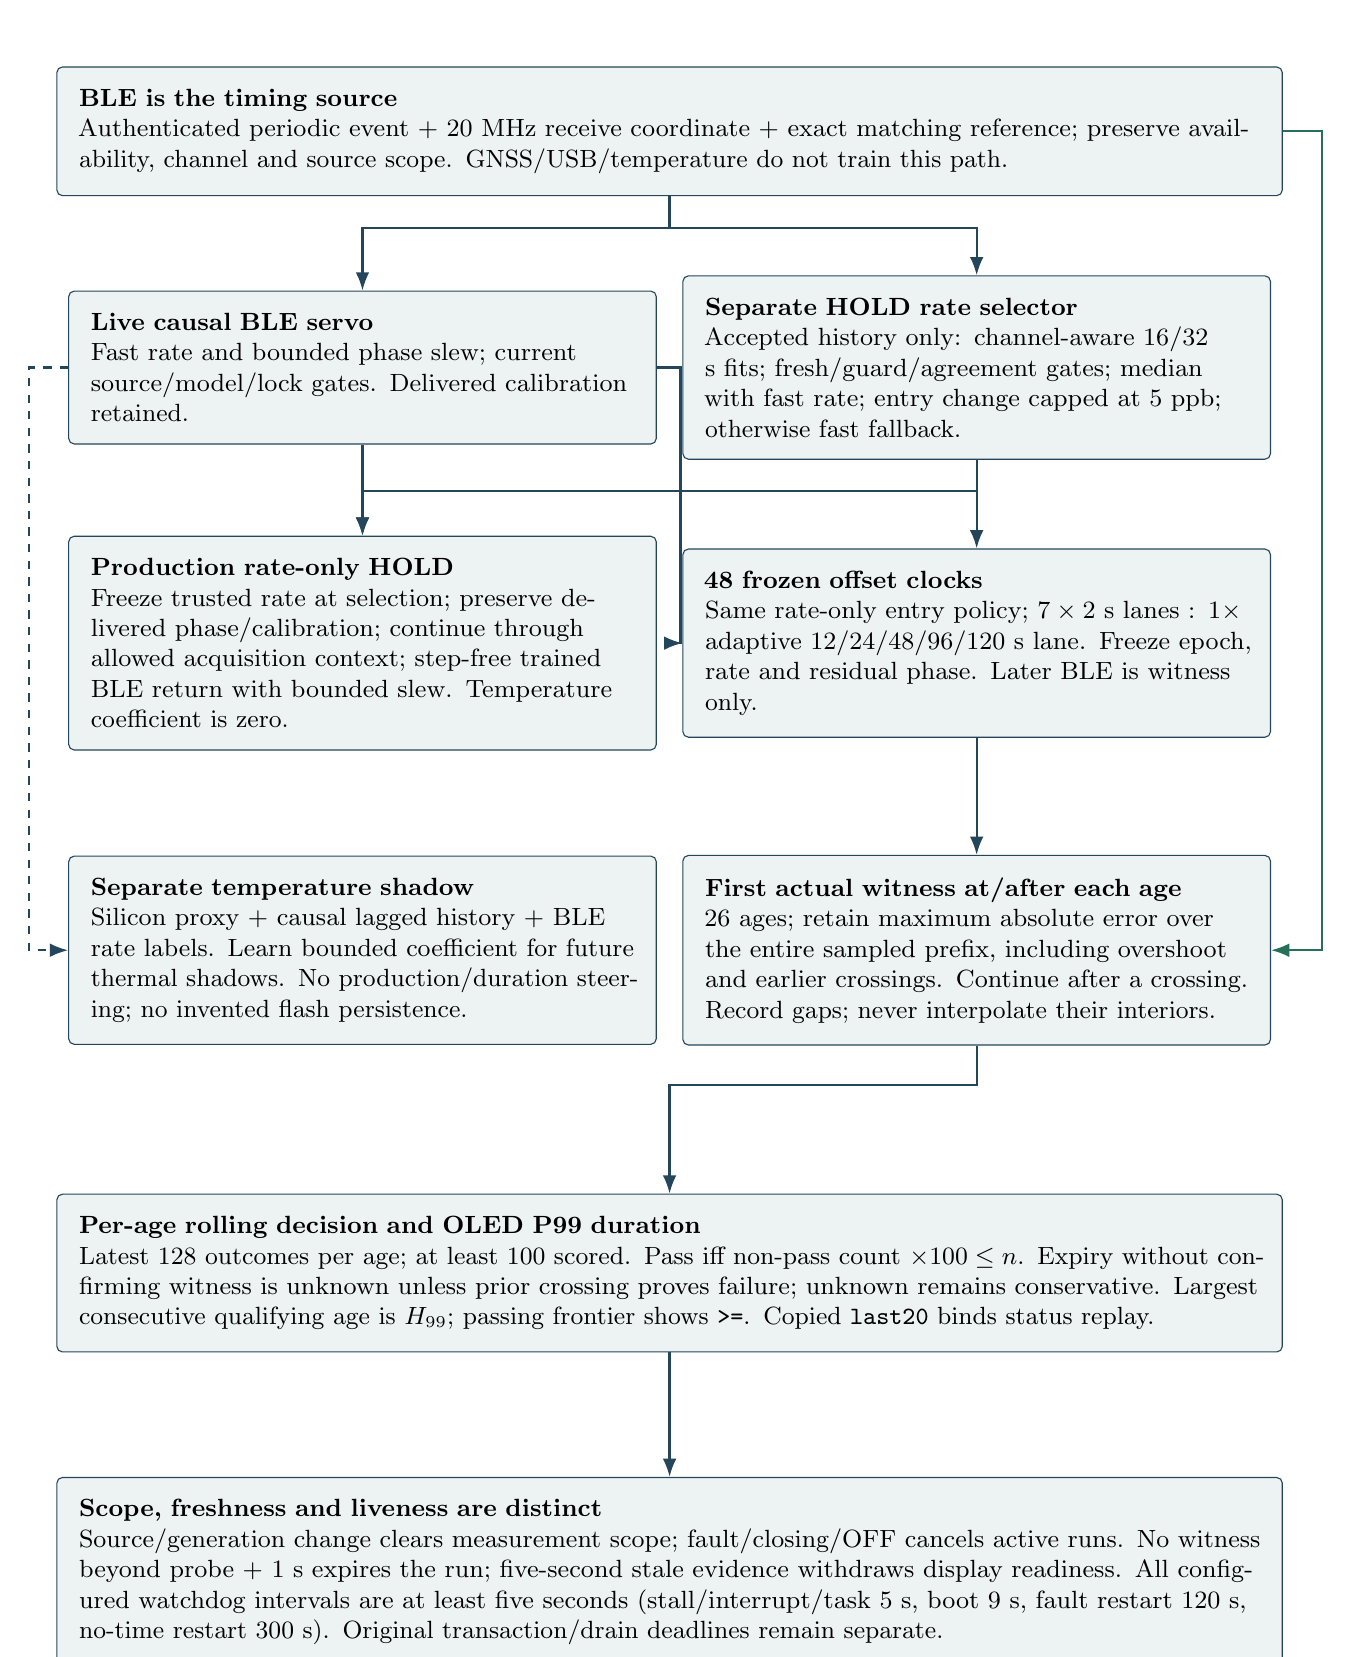
\begin{tikzpicture}[>=Latex,font=\small,box/.style={draw=ink,rounded corners=2pt,fill=pale,align=left,inner sep=8pt},flow/.style={->,draw=ink,line width=.8pt},note/.style={align=left,font=\footnotesize}]
\node[box,text width=150mm](ble) at (0,0){\textbf{BLE is the timing source}\\Authenticated periodic event + 20 MHz receive coordinate + exact matching reference; preserve availability, channel and source scope. GNSS/USB/temperature do not train this path.};
\node[box,text width=69mm](fast) at (-39mm,-30mm){\textbf{Live causal BLE servo}\\Fast rate and bounded phase slew; current source/model/lock gates. Delivered calibration retained.};
\node[box,text width=69mm](rate) at (39mm,-30mm){\textbf{Separate HOLD rate selector}\\Accepted history only: channel-aware 16/32 s fits; fresh/guard/agreement gates; median with fast rate; entry change capped at 5 ppb; otherwise fast fallback.};
\draw[flow](ble.south)--++(0,-4mm)-|(fast.north);\draw[flow](ble.south)--++(0,-4mm)-|(rate.north);
\node[box,text width=69mm](prod) at (-39mm,-65mm){\textbf{Production rate-only HOLD}\\Freeze trusted rate at selection; preserve delivered phase/calibration; continue through allowed acquisition context; step-free trained BLE return with bounded slew. Temperature coefficient is zero.};
\node[box,text width=69mm](shadow) at (39mm,-65mm){\textbf{48 frozen offset clocks}\\Same rate-only entry policy; $7\times2$ s lanes : $1\times$ adaptive 12/24/48/96/120 s lane. Freeze epoch, rate and residual phase. Later BLE is witness only.};
\draw[flow](fast)--(prod);\draw[flow](rate.south)--++(0,-4mm)-|(prod.north);\draw[flow](rate)--(shadow);\draw[flow](fast.east)--++(3mm,0)|-(shadow.west);
\node[box,text width=69mm](temp) at (-39mm,-104mm){\textbf{Separate temperature shadow}\\Silicon proxy + causal lagged history + BLE rate labels. Learn bounded coefficient for future thermal shadows. No production/duration steering; no invented flash persistence.};
\node[box,text width=69mm](score) at (39mm,-104mm){\textbf{First actual witness at/after each age}\\26 ages; retain maximum absolute error over the entire sampled prefix, including overshoot and earlier crossings. Continue after a crossing. Record gaps; never interpolate their interiors.};
\draw[flow](shadow)--(score);\draw[flow,green](ble.east)--++(5mm,0)|-(score.east);
\draw[flow,dashed](fast.west)--++(-5mm,0)|-(temp.west);
\node[box,text width=150mm](rings) at (0,-145mm){\textbf{Per-age rolling decision and OLED P99 duration}\\Latest 128 outcomes per age; at least 100 scored. Pass iff non-pass count $\times100\leq n$. Expiry without confirming witness is unknown unless prior crossing proves failure; unknown remains conservative. Largest consecutive qualifying age is $H_{99}$; passing frontier shows \code{>=}. Copied \code{last20} binds status replay.};
\draw[flow](score.south)--++(0,-5mm)-|(rings.north);
\node[box,text width=150mm](guards) at (0,-183mm){\textbf{Scope, freshness and liveness are distinct}\\Source/generation change clears measurement scope; fault/closing/OFF cancels active runs. No witness beyond probe + 1 s expires the run; five-second stale evidence withdraws display readiness. All configured watchdog intervals are at least five seconds (stall/interrupt/task 5 s, boot 9 s, fault restart 120 s, no-time restart 300 s). Original transaction/drain deadlines remain separate.};
\draw[flow](rings)--(guards);
\end{tikzpicture}
\end{center}
\vspace{-4pt}{\small\textbf{Figure 2.} Final audited v34 dataflow; experimental cohorts remain installed v33. Solid scoring arrows carry observations into the frozen-clock evaluator, never corrections back into held clocks. The schematic follows the supplied current source snapshots and source-scope hooks; measured v30 and v33 cohorts retain their own identities. No physical RF/UTC bound or qualified source handoff is implied.}
\end{document}
